\chapter{Processo}

\section{Gestione dei processi}
\small
\begin{verbatim}
	#include <all.h>
	
	void f1() {
		char_write(`a');
	}
	
	void f2() {
		f1();
	}
	
	void main() {
		natw id = activate_p(f1, 10, 40, LIV_UTENTE);
		terminate_p();
	}
\end{verbatim}
\normalsize
Una delle cose che possiamo fare con questo sistema è gestire i processi.  Il sistema mi fornisce la primitiva \emph{activate$\_$p}, che mi permette di attivare un nuovo processo. Devo indicare
\begin{itemize}
	\item la funzione che dovrà eseguire questo processo,
	\item gli eventuali parametri in ingresso,
	\item la precedenza (si esprime come valore numerico),
	\item il livello di privilegio (in realtà la primitiva non ci concederebbe la creazione di un processo sistema, solo che questa cosa può essere utilizzata dal modulo I/O, che può chiedere di creare un processo a livello sistema).
\end{itemize}
La decisione di quali processi vanno avanti e quando è una delle questioni più bollenti riguardo i sistemi operativi. 
\paragraph{Identificativo del processo} La funzione restituisce un valore: l'identificatore del processo appena creato. Restituisce una sequenza di $1$ nel caso in cui ci siano stati errori.

\paragraph{Che differenza c'è tra \emph{printf} e \emph{writeconsole}?} La \emph{printf} è una libreria di funzione che per stampare caratteri userà delle primitive. La \emph{writeconsole} è una primitiva vera e propria.

\paragraph{Come si realizza l'astrazione dei processi?}
Durante la sua vita un processo può trovarsi in uno tra diversi stati di esecuzione. Il processore sta eseguendo le istruzioni del programma, sta portando avanti lo stato del processo.  Se abbiamo un solo processore solo un processo può trovarsi nello stato \textbf{esecuzione}. Tutti gli altri processi presenti nel sistema possono trovarsi in uno tra i seguenti stati:
\begin{itemize}
	\item \textbf{pronti} (il processo potrebbe andare avanti se dipendesse solo da lui, non va avanti perché il processore è già occupato da qualcun'altro con precedenza maggiore),
	\item \textbf{bloccati} (il processo sta attendendo il verificarsi di un certo evento, per esempio il termine di un'operazione di I/O, non può andare avanti neanche col processore libero).
\end{itemize}
Supponiamo di avere due processi: \emph{job1} e \emph{job2}, il primo ha precedenza maggiore.
\begin{center}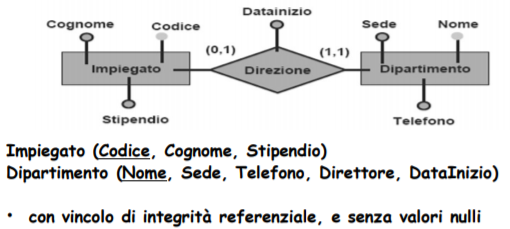
\includegraphics[scale=.75]{img/127.PNG}\end{center}
\begin{itemize}
	\item Si inizia con l'esecuzione di \emph{job1}, che ha priorità maggiore. Rimane in stato \emph{esecuzione} finchè non avvia l'operazione di I/O output. A quel punto il \emph{job1} si pone nello stato \emph{bloccato} e passa la palla a \emph{job2}.
	\item Il processo \emph{job2} passa in \emph{esecuzione}. Si eseguono istruzioni finchè l'operazione di I/O non risulta completata. A quel punto si ha una richiesta di interruzione intercettata dal sistema: la routine rimette \emph{job1} in \emph{esecuzione} e pone \emph{job2} nello stato \emph{pronto}.
	\item Il processore conclude l'esecuzione di \emph{job1} invocando una primitiva di sistema: a quel punto si rimette in \emph{esecuzione} il processo \emph{job2}.
\end{itemize}
I passaggi sono intramezzati per forza di cose, abbiamo numerose variazioni di stato dei vari processi. Si parla di:
\begin{center}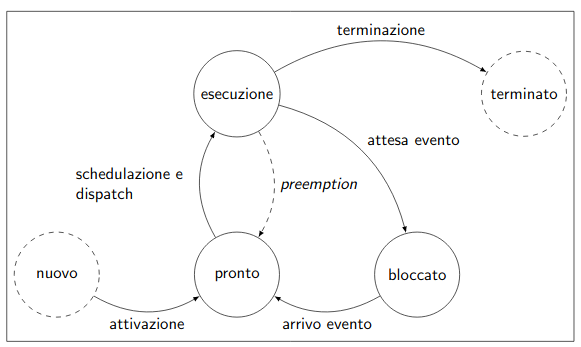
\includegraphics[scale=.76]{img/198.PNG}\end{center}
\begin{itemize}
	\item \textbf{schedulazione}, quando un processo passa da \emph{pronto} a \emph{esecuzione};
	\item \textbf{blocco}, quando un processo passa da \emph{esecuzione} a \emph{bloccato};
	\item \textbf{risveglio}, quando un processo passa da \emph{bloccato} a \emph{esecuzione};
	\item \textbf{preemption}, quando un processo passa da \emph{esecuzione} a \emph{pronto},.
\end{itemize}
L'ultimo passaggio, che possiamo italianizzare in \emph{prelazione}, avviene quando è possibile eseguire processi con priorità maggiore. La cosa non è presente in tutti i sistemi multiprocesso.
\paragraph{Conseguenza di questa assenza}  Un processo va avanti finchè non si blocca, ma per bloccarsi è lui che chiama una primitiva di sistema. Se fa un ciclo infinito il processore rimane lì. Se c'è un errore in un programma  tutto il sistema si blocca (ripensare a sistemi operativi come \emph{Windows 95 / 98 / ME}). In un sistema del genere il processore si accorge di processi con priorità maggiore solo dopo che il processo in esecuzione è stato bloccato.
\paragraph{Creazione di processi} Un processo può creare altri processi assegnando una priorità minore o maggiore. Se il processo ha priorità maggiore potrebbe fare \emph{preemption} subito. Nel nostro caso non sarà così perché imporremo la creazione di processi aventi priorità minore.
\paragraph{Terminazione dei processi} Il processo può essere terminato solo mediante esecuzione di primitiva, dunque il processo dovrà essere in \emph{esecuzione}. Per permettere a processi di uccidere altri processi dobbiamo implementare ulteriori meccanismi che non ci interessano. Distinguiamo la cosa da una terminazione dovuta a eccezioni.

\paragraph{Sistema come intermediario} I cambi di processo avvengono grazie all'intermediazione del sistema: avvengono solo quando i processi, che normalmente girano a livello utente, sono passati a livello sistema (con uno dei metodi possibili, per eccezione, interruzione esterna o istruzione INT). Tutto ciò è vero per tutti i sistemi multiprogrammati. 

\paragraph{Semplificazioni} Il nostro sistema adotta alcune semplificazioni:
\begin{itemize}
	\item una schedulazione che si basa solo sulle precedenze dei processi;
	\item il sistema è multiprocesso ma non multiutente.
\end{itemize}
La multiprogrammazione si è resa necessaria andando avanti: è vero che l'utente è unico, ma è vero che l'utente singolo vuole fare più cose in simultanea. L'utente, inoltre, esegue programmi non realizzati da lui, ed esegue in simultanea programmi realizzati da sviluppatori diversi.
\clearpage 

\section{Processo dal punto di vista dell'utente}
Un'altra cosa su cui i sistemi possono distinguersi è quanta memoria i processi possono condividere tra di loro (condividere nel senso avere processi con dati in comune). Abbiamo sistemi \emph{a scambio di messaggi} (dove non si condivide niente) e sistemi \emph{a memoria comune} (dove condividono tutto). Quello che faremo noi è un ibrido.
\begin{itemize}
	\item \textbf{Parte condivisa}. 
	
	I processi condividono tutto ciò che è globale nel modulo utente
	\begin{verbatim}
		.text
		.data
		.bss
		.heap // anche lo heap, creato a tempo di esecuzione
	\end{verbatim}
	\item \textbf{Parte non condivisa}.
	
	Ogni processo presenta una \emph{pila privata}.
\end{itemize}
Le pile sono separate in modo netto: un processo non ha la possibilità di accedere alla pila di un altro processo.

\section{Processo dal punto di vista del programmatore}
Dal punto del sistema abbiamo un programmatore, non un utente, che prepara le strutture dati e le routine necessarie per realizzare quanto visto dall'utente. Ogni processo è descritto da una \emph{struct}: il \textbf{descrittore di processo}
\begin{verbatim}
	des_proc *pronti;
	des_proc *esecuzione; // <--- uno solo, visto che abbiamo solo un processore
	const int N_REG = 16;
	
	struct des_proc {
		natw id;
		natw livello;
		natl precedenza;
		vaddr punt_nucleo; /* Puntatore a pila sistema */
		natq contesto[N_REG];
		paddr cr3;
		
		des_proc *puntatore;
	};
\end{verbatim}
\begin{itemize}
	\item \textbf{esecuzione}. Una variabile globale (il puntatore \emph{esecuzione}) si ricorda del processo in esecuzione (ricordiamo, uno solo se abbiamo un solo processore).
	\item \textbf{punt$\_$nucleo}. Il sistema oltre ad avere un descrittore di processo per ogni processo ha anche una pila sistema diversa per ogni processo. perché? Abbiamo detto che ogni processo deve avere la sua pila: la cosa è valida non solo in modalità utente, ma anche in modalità sistema. Tutte le informazioni che il processore salva quando attraversa un gate devono rimanere sulla pila del processo, poichè costituiscono lo stato del processo quando si verifica l'interruzione/eccezione/int (tutte cose che dobbiamo tenere da parte).
	\item \textbf{contesto}. La cosa più importante che il sistema deve ricordarsi, di ogni processo, è "l'ultima foto" del suo sistema, che consiste in particolare nel contenuto dei registri. Abbiamo un array \emph{contesto} nella struttura, che contiene il valore corrente di tutti i registri del processore (ci semplifichiamo la vita non memorizzando lo stato della memoria).
	\item \textbf{puntatore}. All'interno della struttura abbiamo \emph{puntatore}, un puntatore necessario per costruire delle liste che rappresentano tutti i processi che si trovano nei vari stati. 
	\begin{itemize}
		\item \textbf{pronti}. Tutti i processi pronti si trovano in una lista: il nostro sistema avrà una variabile globale (il puntatore \emph{pronti}) che punta al primo elemento della lista. I vari elementi che costituiscono la lista sono le strutture \emph{des$\_$proc}. La lista è ordinata in base al campo \emph{precedenza} del processo, segue che per l'operazione di \emph{schedulazione} basterà leggere il primo elemento della lista (cosa con complessità nulla).
		\item Esistono più liste dedicate ai processi bloccati, ciascuna riguardante uno specifico evento: lista per chi aspetta di utilizzare l'hard disk, chi la tastiera, chi il timer...
	\end{itemize}
	Queste liste sono gestite dal sistema, dopo aver ottenuto nuovamente il controllo a seguito del passaggio del gate (ricordiamoci, serve l'atomicità per manipolare delle liste).
	\item \textbf{cr3}. Affrontato più avanti, nel capitolo sulla paginazione.
\end{itemize}
\paragraph{Differenze tra routine di sistema e routine di interruzione} 
\begin{itemize}
	\item Possiamo immaginarci una routine di sistema come una routine di interruzione.
	\item La differenza sostanziale sta nella proprietà di \emph{atomicità} della routine di sistema, ossia la sua indivisibilità. \textbf{La routine di interruzione può essere interrotta da un'altra interruzione, la routine di sistema no}!
	\item \textbf{La routine di sistema non può essere considerata parte del processo} poichè non contribuisce all'avanzare dello stato del processo stesso.
\end{itemize}
\subsection{Passaggio a contesto sistema} Quando il processo passa il gate viene fotografato lo stato del processo corrente.  Il passaggio al \emph{contesto sistema} avviene con il seguente codice Assembler
\begin{verbatim}
	CALL salva_stato
	// ...
	// codice della routine di sistema
	// ...
	CALL carica_stato
	IRETQ
\end{verbatim}
\begin{itemize}
	\item Con la \emph{salva$\_$stato} è una routine scritta in assembler che salva, nel campo \emph{contesto} del processo in esecuzione, lo stato dei registri.
	\item Questo codice in realtà è il solito incapsulamento che abbiamo già usato altre volte. Non ci piace programmare in Assembler, dunque tra le due call chiameremo una routine implementata in C++. Ricordarsi che l'incapsulamento via Assembler è obbligatorio a causa della IRETQ (come la chiamiamo in C++? Non si può).
	\item Con la \emph{carica$\_$stato} poniamo il contenuto del campo \emph{contesto} (del processo in esecuzione) nei vari registri.
\end{itemize}
\paragraph{Ribadiamo}
\[\boxed{\text{Quanto posto tra le due call non deve essere considerato parte del processo.}}\]
\subsection{Passaggio da un processo a un altro attraverso routine di sistema} Il passaggio da un processo a un altro è cosa semplice a questo punto. Abbiamo un codice simile al precedente (il passaggio avviene mediante routine di sistema, visto che il tutto funzione con l'intermediazione del sistema)
\begin{verbatim}
	CALL salva_stato
	// ...
	esecuzione = ...
	// ...
	CALL carica_stato
	IRETQ
\end{verbatim}
ma modifichiamo tra le due call il valore del puntatore \emph{esecuzione} (il valore precedente sarà posto in un'altra coda). Quando la nostra routine di sistema finisce la \emph{carica$\_$stato}  andrà a porre nei registri il \emph{contesto} del nuovo processo puntato dalla variabile globale \emph{esecuzione} (\textbf{solo a questo punto avviene il passaggio}).

\paragraph{Memoria protetta} Dal punto di vista della protezione tutte queste strutture dati (descrittori di processo, pile di sistema, variabili globali \emph{pronti} ed \emph{esecuzione}) devono stare nella parte di memoria non accessibile agli utenti. Distinguiamo due aree di memoria:
\begin{itemize}
	\item le strutture dati, i descrittori di processo, le pile sistema stanno nell'area di memoria non accessibile all'utente;
	\item modulo utente e pila del processo corrente stanno nell'area accessibile all'utente (supponiamo ci sia una pila alla volta in memoria).
\end{itemize}

\subsection{Atomicità: perché la routine di sistema deve essere indivisibile?} 
Dal punto di vista della correttezza limitarsi a proteggere una parte di memoria non è sufficiente. Dobbiamo garantire l'\emph{atomicità} per evitare problemi.
%\paragraph{Premessa} Ricordiamo quanto visto nella lezione del 15 aprile. Abbiamo un programma principale, un'interruzione, una variabile \emph{fine} letta dal programma principale e modificata dalla routine di interruzione.
%\begin{center}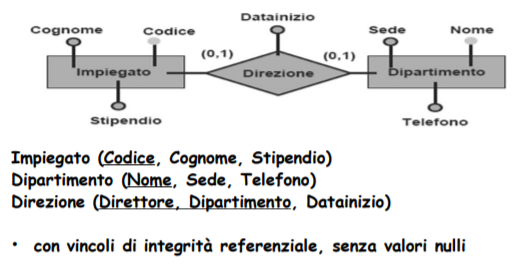
\includegraphics[scale=.55]{img/128.PNG}\end{center}
%La cosa si risolve ponendo la keyword \emph{volatile}. Quanto detto è il caso più semplice di condivisione di variabili tra due flussi di controllo non sequenziali (cioè due flussi mescolabili in maniera arbitraria). Gestire le interruzioni non è cosa semplice, e nel caso di routine di sistema può provocare problemi. 
\paragraph{Singole istruzioni} Un'istruzione è per definizione indivisibile: abbiamo detto che le interruzioni si manifestano tra un'istruzione e un'altra, non durante l'esecuzione di una singola istruzione.
\paragraph{Consistenza delle liste} Prendiamo ad esempio la gestione delle liste con i processi, che è in mano al sistema (l'intermediario, prendiamo ad esempio la coda \underline{globale} \emph{pronti}). 
\begin{center}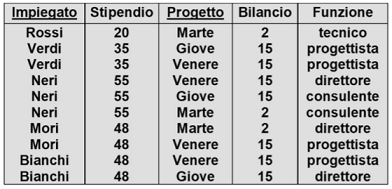
\includegraphics[scale=.65]{img/129.PNG}\end{center}
Abbiamo visto che la manipolazione della lista non richiede una semplice istruzione macchina, ma una serie di istruzioni durante le quali la lista non è consistente. La lista è consistente all'inizio (prima delle modifiche) e alla fine (dopo le modifiche). Lanciare un'interruzione nel bel mezzo della sua manipolazione significa considerarla in uno stato inconsistente (si hanno problemi se mentre stiamo manipolando una lista si ha un'interruzione e la relativa routine interviene anch'essa sulla lista che era in corso di modifica).  Ricordarsi che
\[\boxed{\text{La lista è consistente solo se tutti gli elementi sono raggiungibili partendo dalla testa}}\]
\paragraph{Cosa facciamo?} Seguono due strade possibili:
\begin{enumerate}
	\item scrivere le routine pensando al fatto che lo stato considerato possa essere inconsistente (il programmatore normalmente scrive pensando che nessuno si metta di mezzo tra le istruzioni del suo programma);
	\item impedire le interruzioni in modo tale che gli stati inconsistenti non siano visibili.
\end{enumerate}
La prima cosa è dispendiosa, la seconda semplice:
\begin{itemize}
	\item per le interruzioni esterne si ricorre a un apposito flag (il flag IF);
	\item le eccezioni devono essere evitate dal sistema;
	\item stessa cosa le interruzioni software (ad ogni chiamata di routine corrisponde una \emph{salva$\_$stato}, che sovrascrive il contesto precedente\footnote{Ricordiamo che ciò che viene eseguito in una routine di sistema non è parte di un processo. L'esecuzione di una \emph{salva$\_$stato} comporta la perdita delle informazioni relative alla routine eseguita.}).
\end{itemize}
In questo modo evitiamo tutti i meccanismi che permettono di attraversare il gate e di ritornare ricorsivamente nel sistema. Possiamo dire che \textbf{la routine di sistema è diventata, in un certo senso, simile a un'unica istruzione di linguaggio macchina} (è atomica e indivisibile, viene eseguita fino alla sua fine). 

\paragraph{Wait, altro problema} Tenere disattivate le interruzioni \underline{è una limitazione troppo grande} per molti progettisti di sistema, dunque si è elaborata una via di mezzo. Nel modulo I/O, che vedremo più avanti, abbiamo un rilassamento delle restrizioni:
\begin{itemize}
	\item le eccezioni sono normalmente vietate;
	\item le interruzioni sono ammesse;
	\item la chiamate ricorsive sono permesse (forse si, forse no).
\end{itemize}
Tutto rimane vietato nel modulo sistema (atomicità, per forza).

\subsection{Prima istantanea dello stato di un processo} Per i processi appena partiti non è mai stata scattata una foto prima. La foto viene scattata quando si entra in modalità sistema: meccanismo delle eccezioni, processore (salva le informazioni nella pila sistema privata, per la IRETQ), in parte con la \emph{salva$\_$stato} (si aggiorna la struttura \emph{des$\_$proc}). Tutto questo funziona quando il processo esiste già e si attraversa un gate: ma per i processi appena creati? Il modo più semplice è fare in modo che l'\emph{activate$\_$p} generi la foto: 
\begin{verbatim}
	activate_p(miaproc, 10, 20, LIV_UTENTE);
\end{verbatim}
questo significa creare l'istanza relativa della struttura \emph{des$\_$proc} e allocare la pila di sistema.
\begin{itemize}
	\item Intanto posso impostare in \emph{des$\_$proc} la priorità e il livello di privilegio.
	\item Successivamente devo inizializzare il contesto e la pila in modo tale che le seguenti istruzioni, eseguite da una qualche routine, diano inizio al processo in modo regolare.
	\begin{verbatim}
		CALL carica_stato
		IRETQ
	\end{verbatim}
	\begin{itemize}
		\item In pila mettiamo 5 \emph{quadword} (la IRETQ vuole questo, ricordiamolo). Abbiamo:
		\begin{multicols}{2}
			\begin{itemize}
				\item (RIP) l'indirizzo della funzione da eseguire;
				\item (CPL) si imposta in modo che il livello di privilegio sia quello indicato nell'apposito parametro di ingresso;
				\item (RFLAG), si impostano i flag con IF ad 1 e IOPL sempre \textit{sistema} (si indica il \emph{Privilege level} necessario per eseguire certe istruzioni);
				\item (RSP), si pone l'indirizzo con la pila utente del processo in esecuzione;
				\item (TSS) cose relative ai segmenti che non ci interessano.
			\end{itemize}
			\columnbreak
			\begin{center}
				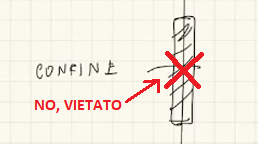
\includegraphics[scale=.8]{img/283.PNG}
			\end{center}
		\end{multicols}
		Si consideri che in un processo a livello sistema si crea solo la pila sistema, mentre in un processo a livello utente si crea sia la pila sistema che quella utente.
		\item Il contesto ha almeno due registri da inizializzare in modo preciso, gli altri possono essere uguali a zero.
		\begin{itemize}
			\item Il parametro in ingresso deve andare in RDI (la funzione \emph{miaproc} ha un parametro con valore $10$, lo mettiamo subito nel registro - secondo le regole già viste - per permettere l'esecuzione della funzione).
			\item Dobbiamo mettere in RSP l'indirizzo della pila sistema, in modo tale che IRETQ possa leggere i dati che abbiamo messo nella pila sistema.
		\end{itemize}
	\end{itemize}
	\item Si consideri che l'indirizzo della pila sistema non viene preso da \emph{des$\_$proc} ma da quella roba brutta vista qualche lezione fa: passaggio dal TR (\emph{Task Register}) per arrivare alla GDT (\emph{Global Descriptor Table}) e infine al TSS (\emph{Task State Segment}). Per indicare al processore di usare una certa pila abbiamo due strade...
	\begin{itemize}
		\item \textbf{Un TSS per processo}.
		
		Uso il meccanismo della segmentazione progettato da Intel (quindi \emph{punt$\_$nucleo} punta al TSS) come descrittore di processo (però a quel punto ci serve un TSS per ogni processo e siamo limitati nel numero a causa degli ingressi limitati della GDT) e cambiare ogni volta il valore del registro TR;
		\item \textbf{Un unico TSS per tutti i processi} (soluzione adottata).
		
		Ci limitiamo a creare un solo TSS (quindi il valore del registro TR è costante) per fare contento il processore, e quando cambiamo processo la \emph{carica$\_$stato} prende il puntatore alla pila sistema dal \emph{des$\_$proc} e lo pone nel TSS.
	\end{itemize}
\end{itemize}

\begin{center}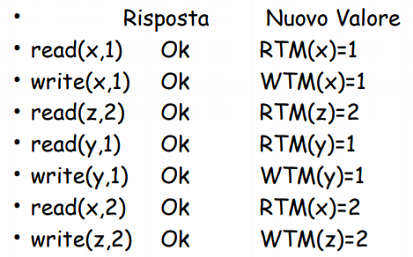
\includegraphics[scale=.65]{img/170.PNG}\end{center}